% This is my super simple Real Analysis Homework template

\documentclass{article}
\usepackage[utf8]{inputenc}
\usepackage[english]{babel}
\usepackage[]{amsthm} % lets us use \begin{proof}
\usepackage[]{amssymb} % gives us the character \varnothing
\usepackage{physics}
\usepackage{fourier-orns}
\usepackage{comment}
%\usepackage[fleqn]{amsmath}
\usepackage{tikz,lipsum}
\usetikzlibrary{arrows,automata}
\usepackage{multicol}
\usepackage{enumitem}
\usepackage{mathtools}
\DeclarePairedDelimiter\ceil{\lceil}{\rceil}
\DeclarePairedDelimiter\floor{\lfloor}{\rfloor}

\title{Leetcode, $\cdots$}
\author{}
\date{}
% This information doesn't actually show up on your document unless you use the maketitle command below

\begin{document}
\maketitle %This command prints the title based on information entered above

\section*{Critical Connections in a Network}
% For fancy calligraphy letters, use \mathcal{}
\textbf{id}: 1192 \quad tags: graph, dfs \\
\textbf{Par}
\begin{tabular}{ll}
    \texttt{ids[node]}      & keep tracking ids of nodes in dfs ordering \\
    \texttt{low[node]}      & smallest id which current node can reach \\
    \texttt{graph[node]}    & adjacency list \\
\end{tabular}
\\ \textbf{Alg}
\begin{enumerate}
\item
    build graph in form of adjacency list, \texttt{graph[node]}
\item
    tranverse graph dfsly. If neighbor node is not visited, dfs next node, update \texttt{low[node]} by \texttt{min(low[node], low[neighbor])} by callback.
\item
    Check if \texttt{ids[node] < low[neighbor]} is true, then we find one critical connection. 
\item
    If neighbor node is visited and it is not the node visited right before current node, update \texttt{low[node]} by the same as in 2.

\end{enumerate}
\begin{multicols}{2}
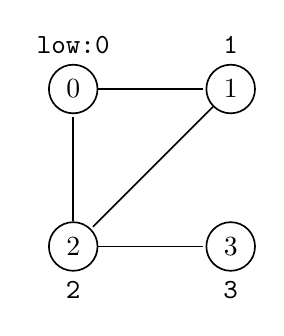
\begin{tikzpicture}[-,>=stealth',shorten >=1pt,auto,node distance=2cm,
                    semithick]
    \tikzset{every state/.style={minimum size=0pt}}
    \node[state,label=above:\texttt{low:0}] (0) {0};
    \node[state,label=above:\texttt{1}] (1) [right of=0] {1};
    \node[state,label=below:\texttt{2}] (2) [below of=0] {2};
    \node[state,label=below:\texttt{3}] (3) [right of=2] {3};
    \path
    (0) edge node{} (1)
    (1) edge node{} (2)
    (2) edge node{} (3)
    (2) edge node{} (0);
\end{tikzpicture}

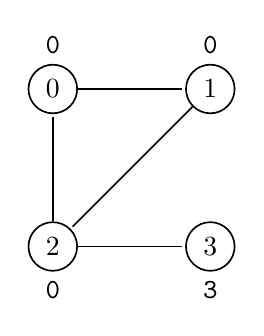
\begin{tikzpicture}[-,>=stealth',shorten >=1pt,auto,node distance=2cm,
                    semithick]
    \tikzset{every state/.style={minimum size=0pt}}
    \node[state,label=above:\texttt{0}] (0) {0};
    \node[state,label=above:\texttt{0}] (1) [right of=0] {1};
    \node[state,label=below:\texttt{0}] (2) [below of=0] {2};
    \node[state,label=below:\texttt{3}] (3) [right of=2] {3};
    \path
    (0) edge node{} (1)
    (1) edge node{} (2)
    (2) edge node{} (3)
    (2) edge node{} (0);
\end{tikzpicture}
\end{multicols}
You can see that \texttt{ids[2] < low[3]}.

\clearpage % Gives us a page break before the next section. Optional.
\section*{Max Sum of Rectangle No Larger Than K }
\textbf{id}: 363 \\
\textbf{tags}: binary search\\
\[
\textbf{Par} \left\lbrace
\begin{tabular}{ll}
    \texttt{mat}    & the original matrix\\
    \texttt{arr}    & array of sums from column $i$ to $j$ of \texttt{mat}\\
    \texttt{sums}   & ordered set of sums from begin to \texttt{arr[i]} \\
    \texttt{cur}    & current sum of \texttt{arr[0$\cdots$i]} \\
    \texttt{k}      & threshold for the result\\
\end{tabular}
\right.
\]
\\
\textbf{Alg}
\begin{enumerate}
\item
    Sub problem: Max sum of subarray of array $arr$ \\
    Init \texttt{sums} with 0, $res$ with $-\infty$.\\
    Iterate \texttt{arr}: at \texttt{i} iteration, \texttt{cur += arr[i]}. \\
    Find the index of lower bound $lb$ of \texttt{cur-k} in \texttt{sums}. \\
    If $lb$ is not the end of \texttt{sums}, we have
        $res = \max(res, \texttt{cur - sums[lb]})$.

\item
    Then we use 
\item
    todo

\end{enumerate}

\clearpage
\section*{Find Peak Element}
\textbf{id}: 363 \\
\textbf{tags}: binary search\\
\[
\textbf{Par} \left\lbrace
\begin{tabular}{ll}
    \texttt{nums}   & array, where \texttt{nums[i] != nums[j]} 
                    if \texttt{i != j} \\
    \texttt{l}      & left pos \\
    \texttt{r}      & right pos \\
    \texttt{m}      & middle = (left+right) / 2\\
\end{tabular}
\right.
\]
\\
\textbf{Alg}
\begin{enumerate}
\item
    init left, right \texttt{l = 0, r = len(nums)-1}
\item
    \texttt{while l < r: \\
        \null\qquad m = (l+r) // 2\\
        \null\qquad if (nums[m] > nums[m+1]: r = m\\
        \null\qquad else: l = m+1}
\item
    the final \texttt{l} is the answer.

\end{enumerate}



\clearpage
\section*{Sample}
\textbf{id}: 363 \\
\textbf{tags}: binary search\\
\[
\textbf{Par} \left\lbrace
\begin{tabular}{ll}
    \texttt{a}   & xxx \\
    \texttt{b}    & xxx \\
    \texttt{c}      & xxx \\
\end{tabular}
\right.
\]
\textbf{Alg}
\begin{enumerate}
\item
    todo
\item
    todo
\item
    todo

\end{enumerate}


\end{document}
